\documentclass[letterpaper]{article}
\usepackage[utf8]{inputenc}
\usepackage[spanish]{babel}
\usepackage{amssymb, amsmath}
\usepackage{graphicx}
\usepackage{lipsum}
\usepackage{dsfont}
\usepackage[margin=1.5cm,
vmargin={1.5cm,1.3cm},
includefoot]{geometry}
\usepackage{setspace}
\usepackage{subcaption}
\usepackage{tocloft}
\usepackage{upgreek}
\usepackage{amsthm}
\usepackage{graphicx}
\usepackage{paralist}
\usepackage{fancyhdr}
\usepackage{lmodern}
\usepackage{tcolorbox}
\usepackage{color}
\usepackage{tikz}
\tcbuselibrary{skins,breakable}
\pagestyle{fancy}

\renewcommand{\headrulewidth}{0.4pt}
\renewcommand{\footrulewidth}{0.4pt}

\providecommand{\abs}[1]{\left|#1\right|}
\providecommand{\norm}[1]{\left|\left|#1\right|\right|}														  
\newcommand{\V}{\mathds{V}}

\newcommand{\W}{\mathds{W}}

\newcommand{\F}{\mathds{F}}

\newcommand{\tq}{ \quad \cdot  \backepsilon \cdot \quad }

\newcommand{\ld}{\lim\limits_{x \to 0^{+}}}

\newcommand{\li}{\lim\limits_{x \to 0^{-}}}

\newcommand{\la}{\lim\limits_{x \to a}}

\newcommand{\R}{\mathds{R}}

\newcommand{\Po}{\mathds{P}_2(\mathds{R})}

\renewcommand{\*}{\cdot}

\newcommand{\Iden}{\begin{pmatrix}
		1 & 0 & 0\\
		0 & 1 & 0\\
		0 & 0 & 1 
\end{pmatrix}}
\newcommand{\T}{\begin{pmatrix}
		1 & 3 & 9 \\
		1 & 3 & 4 \\
		0 & 0 & 2 
\end{pmatrix} }

\makeatletter
\renewcommand*\env@matrix[1][*\c@MaxMatrixCols c]{%
	\hskip -\arraycolsep
	\let\@ifnextchar\new@ifnextchar
	\array{#1}}
\makeatother

\newtheorem{theorem}{Teorema}[section]
\theoremstyle{definition}
\newtheorem{definition}{Definición}

\begin{document}
	
	\setlength{\unitlength}{1cm}
	\thispagestyle{empty}
	\begin{picture}(19,3)
	\put(-0.5,1.2){
\includegraphics[scale=.20]{unam1.png}}
	\put(16,1){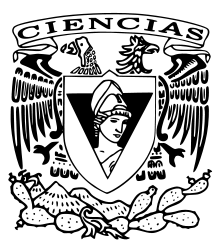
\includegraphics[scale=.29]{fciencias1.png}}
	\end{picture}
	
	\begin{center}
		\vspace{-114pt}
		\textbf{\large Matemáticas para las Ciencias II}\\
		\textbf{ Semestre 2020-2}\\
		Prof. Pedro Porras Flores\\
		Ayud. Irving Hernández Rosas \\
		\textbf{Proyecto III}\\[0.2cm]
		Kevin Ariel Merino Peña\footnote{317031326}\\ [0.2cm]
	\end{center}
	\vspace{-10pt}
	\rule{19cm}{0.3mm}


\noindent Realice los siguientes ejercicios, escribiendo el procedimiento claramente. Y recuerden que estos proyectos se entregan de manera individual en la plataforma de google classroom. \\[0.5cm]
1.  Muestre que los siguientes conjuntos del plano son abiertos: 
\begin{definition}
	Sea $ \vec{x}_0  \in \R^n$  y sea $ r \in \R^+ $, la \textbf{bola} de radio r y centro en $ \vec{x}_0 $ es definida por el conjunto de todos los puntos $ \vec{x} $ tal que $ \norm{\vec{x} - \vec{x}_0} < r $.\\ Este conjunto es denotado como $ Br(\vec{x}_0) $ es el conjunto de los puntos $ \vec{x} \in \R^n $ cuya distancia de $ \vec{x}_0 $ es menor que $ r $
\end{definition}

\begin{definition}
	Sea $ U \subset \R^n $. Decimos que $ U $ es \textbf{conjunto abierto} si para cada $ \vec{x}_0 $, existe algún $ r>0 $ tal que $ Br(\vec{x}_0) $ está totalmente contenida en $ U $, $ Br(\vec{x}_0) \subset U $

\end{definition}

$$\text{a) } A = \{ (x,y) \in \mathbb{R}^2 \vert - 1 < x < 1, - 1 < y < 1 \}$$

$$\text{b) }B = \{ (x,y) \in \mathbb{R}^2 \vert \,  0 < y  \}$$

$$\text{c) }A = \{ (x,y) \in \mathbb{R}^2 \vert \, 2 < x^2  + y^2 <  4 \}$$\\[0.5cm]
2.  Calcule los siguientes. límites si existen: 
\begin{definition}
	Sea $ f: A \subset \R^n \to \R^m $ y $ \vec{x}_0 \in A $, un punto de acumulación de $ A $. Entonces se dice qe el límite de $  f(\vec{x}) $, cuando $ \vec{x} $ tiende a $ \vec{x}_0 $, es $ \vec{\textit{l}} \in \R^m $ y se denota
	\[ \lim\limits_{\vec{x} \to \vec{x}_0} = \vec{\textit{l}} \qquad \text{ o } f(\vec{x}) \to \vec{\textit{l}} \]
	Si $ \forall \epsilon > 0, \quad \exists  \delta > 0 $ tal que $ \vec{x} \to \vec{x}_0 $
\end{definition}


\noindent$\text{a) }\displaystyle\lim_{(x,y) \to (0,0)} \dfrac{\cos(xy) - 1}{x^2y^2}$\\
Resultará conveniente recordar de nuestro curso de Matemáticas para las ciencias aplicadas I que $$ \lim\limits_{\alpha \to 0} \dfrac{cos(\alpha) - 1}{\alpha^2} = -\dfrac{1}{2} $$.  
Entonces tomemos el siguiente cambio de variable $ \alpha = xy $
y por el recordatorio anterior, tenemos que 
 
$$\displaystyle\lim_{(x,y) \to (0,0)} \dfrac{\cos(xy) - 1}{x^2y^2} = -\dfrac{1}{2}$$

\noindent$\text{b) }\displaystyle\lim_{(x,y) \to (0,0)} \dfrac{\sin(xy) }{xy}$\\
Para este segundo ejercicio, tomemos un cambio de variable $ y =\sqrt{r}  $ y $ x = \sqrt{r} $ entonces $ xy = r $ por lo que
$$\text{b) }\displaystyle\lim_{(r\to 0} \dfrac{\sin(r) }{r}$$
Y de nuestro curso de Matemáticas para las ciencias aplicadas I tenemos que $ \lim\limits_{\alpha \to 0} \dfrac{sin(\alpha)}{\alpha} = 1 $, por lo tanto
$$\displaystyle\lim_{(x,y) \to (0,0)} \dfrac{\sin(xy) }{xy} = 1$$

$$\text{c) }\displaystyle\lim_{x \to 1} (x^2 , e^x) $$\\[0.5cm]
Tenemos un teorema enunciado en clase sobre las propiedades de los límites, una de ellas dice:
\begin{definition}
	Si $ f(\vec{x}) = (f_1(\vec{x}), \dots, f_m(\vec{x})) $ donde $ f_i:A \to \R  $, $ i \in \{ 1, \dots, m \} $  son las componentes de la función de $ f $, entonces 
	\[ \lim\limits_{\vec{x} \to \vec{x}_0 } f(\vec{x}) = (l_1, l_2, \dots, l_m) \] si y sólo si\[ \lim\limits_{\vec{x} \to \vec{x}_0} f_i(\vec{x}) = l_i \] para cada $ i \in \{ 1, 2, \dots, m \} $
\end{definition}
entonces si
\begin{align*}
	\lim_{x \to 1} (x^2 , e^x) &=\left( \lim_{x \to 1} x^2, \lim_{x \to 1} e^x \right)\\
	\lim_{x \to 1} (x^2 , e^x) &=\left( (1)^2,  e^{1} \right)\\
	\lim_{x \to 1} (x^2 , e^x) &=\left( 1,  e \right)\\
\end{align*}

3.  Usando la formulación $\epsilon$-$\delta$ muestre: \\

 $$ \text{a) } \displaystyle\lim_{(x,y,z) \to (0,0,0)} \dfrac{xyz}{x^2 + y^2 + z^2} = 0$$\\

$$\text{b) }\displaystyle\lim_{(x,y) \to (0,0)} \dfrac{xy }{\sqrt{x^2 + y^2}} = 0$$\\

$$\text{c) }\displaystyle\lim_{x \to 2} (3x , x^2) = (6,4) $$\\[0.5cm]
4.  Sea $f: \mathbb{R}^2  \longrightarrow \mathbb{R}$ tal que $f(x,y) = \left\{
     \begin{array}{cl}
       \dfrac{x^2y}{\vert x \vert^3 + y^2} & : \text{ si } (x,y) \neq (0,0)\\
       0 & : \text{ si } (x,y) = (0,0)\\
     \end{array}
   \right.$ \\Muestre que $f$ es continua en $(0,0)$
Para averiguar quién es el límite, tomémonos traectorias distintas. \\
Deifinimos $ y = g(x) = 0 $
\begin{align*}
	\lim\limits_{(x,y)\to (0,0)} f(x,y) &= \lim\limits_{(x,y) \to (0,0)} f(x,g(x))\\
	\lim\limits_{(x,y)\to (0,0)} f(x,y) &= \lim\limits_{(x,y) \to (0,0)} f(x,0)\\
	\lim\limits_{(x,y)\to (0,0)} f(x,y) &= \lim\limits_{x \to 0} \dfrac{x^2y}{\vert x \vert^3 + y^2} \\
	\lim\limits_{(x,y)\to (0,0)} f(x,y) &= \lim\limits_{x \to 0} \dfrac{x^2(0)}{\vert x \vert^3 + (0)^2} \\
	\lim\limits_{(x,y)\to (0,0)} f(x,y) &= 0
\end{align*}
Por otra parte, definamos $ y = g(x) = x$ por lo que
\begin{align*}
	\lim\limits_{(x,y)\to (0,0)} f(x,y) &= \lim\limits_{(x,y) \to (0,0)} f(x,g(x))\\
	\lim\limits_{(x,y)\to (0,0)} f(x,y) &= \lim\limits_{(x,y) \to (0,0)} f(x,x)\\
	\lim\limits_{(x,y)\to (0,0)} f(x,y) &= \lim\limits_{x \to 0} \dfrac{x^3}{\vert x \vert^3 + x^2} \\
	\lim\limits_{(x,y)\to (0,0)} f(x,y) &= \lim\limits_{x \to 0} \dfrac{x^3}{x^2  \left( \dfrac{\abs{x}^3}{x^2} + 1 \right) } \\
	\lim\limits_{(x,y)\to (0,0)} f(x,y) &= \lim\limits_{x \to 0} \dfrac{x}{\dfrac{\abs{x}^3}{x^2} + 1 } \\
	\lim\limits_{(x,y)\to (0,0)} f(x,y) &=  \dfrac{\lim\limits_{x \to 0} x}{\lim\limits_{x \to 0} \left( \dfrac{\abs{x}^3}{x^2} + 1 \right) } \\
	\lim\limits_{(x,y)\to (0,0)} f(x,y) &=  \dfrac{\lim\limits_{x \to 0} x}{\lim\limits_{x \to 0}  \dfrac{3\abs{x}^2 \abs{x}'}{2x} + 1  }  && \text{Aplicando ley de L'Hôpital}\\
	\lim\limits_{(x,y)\to (0,0)} f(x,y) &=  \dfrac{\lim\limits_{x \to 0} x}{ \dfrac{3}{2} \lim\limits_{x \to 0}  \dfrac{\abs{x}^2}{x}\* \lim\limits_{x \to 0} \abs{x}'  + 1  }  && \text{Por la regla del producto}\\
	\lim\limits_{(x,y)\to (0,0)} f(x,y) &=  \dfrac{\lim\limits_{x \to 0} x}{ \dfrac{3}{2} \* 0\{-1,1\}  + 1  }  && \text{Por definición de la derivada del valor absoluto }\\
	\lim\limits_{(x,y)\to (0,0)} f(x,y) &=  \dfrac{\lim\limits_{x \to 0} x}{1}  && \text{}\\
	\lim\limits_{(x,y)\to (0,0)} f(x,y) &=  0 && \text{}\\
\end{align*}
Sea $ \epsilon > 0 $, consideremos $ \norm{f(x,y) - l} $, donde $ f(x,y) = \dfrac{x^2y}{\vert x \vert^3 + y^2} $ y $ l = 0 $, entonces
\begin{align*}
	\norm{\dfrac{x^2y}{\vert x \vert^3 + y^2} - 0} &= \abs{\dfrac{x^2y}{\vert x \vert^3 + y^2}} \leq \abs{\dfrac{x^2y}{x^2}}
\end{align*}
luego, veamos que $ \abs{\dfrac{x^2y}{x^2}} = \abs{y} = \sqrt{y^2} $ y como $ 0 \leq y^2 \leq y^2 + x^2 $ tenemos que
\begin{align*}
	\abs{\dfrac{x^2y}{\abs{x}^3 + y^2}} &\leq \abs{y} = \sqrt{y^2}\\
	\abs{\dfrac{x^2y}{\abs{x}^3 + y^2}} &\leq \sqrt{y^2}\\
	\abs{\dfrac{x^2y}{\abs{x}^3 + y^2}} &\leq \sqrt{y^2} \leq \sqrt{x^2 + y^2}\\
	\abs{\dfrac{x^2y}{\abs{x}^3 + y^2}} &\leq \sqrt{y^2} \leq \sqrt{x^2 + y^2} && \text{Puesto que }\sqrt{x^2 + y^2} = \norm{(x,y)} \\
	\abs{\dfrac{x^2y}{\abs{x}^3 + y^2}} &\leq \sqrt{y^2} \leq \norm{(x,y)} < \epsilon && \text{Por hipótesis} \\
	\abs{\dfrac{x^2y}{\abs{x}^3 + y^2}} &\leq \norm{(x,y)} < \epsilon \\
\end{align*}
Por lo tanto, basta tomar $ \delta = \epsilon $





\end{document}
